
\documentclass[aspectratio=169]{beamer}
\usetheme[numbering=fraction,progressbar=frametitle]{metropolis}



% Fonts and symbols
\usepackage{amsmath,amssymb,amsfonts,bm}
\usepackage{mathtools}
\usepackage{physics}
\usepackage{booktabs}
\usepackage{tikz}
\usetikzlibrary{arrows.meta,positioning,fit,calc,shapes.multipart}

% Colors (subtle crypto accents)
% \definecolor{crypto}{RGB}{0,85,164} % deep blue
\definecolor{verifier}{RGB}{0,128,96} % green
\definecolor{issuer}{RGB}{156,39,176} % purple
\definecolor{client}{RGB}{230,81,0} % orange
% \setbeamercolor{frametitle}{fg=crypto}
% \setbeamercolor{progress bar}{fg=crypto,bg=black!10}

\title{Privacy-Preserving Age Verification Using Zero-Knowledge Proofs}
\author{Ali Daher \and Ali Khalil}
\institute{Department of Computer Science, American University of Beirut}
\date{}

\begin{document}

\maketitle

% 1. Problem & Goal
\begin{frame}{Problem \& Goal}
\begin{itemize}
  \item Online services need age checks without exposing personal data. (Privacy, tracking, over-collection)
  \item Goal: Prove ``age $\geq$ threshold'' and validity, with \textbf{no identity leakage} and \textbf{unlinkability}.
  \item Approach: Combine Pedersen commitments, BBS+ signatures (BLS12-381), Bulletproofs, and RSA-accumulator revocation.
\end{itemize}
\end{frame}

% 2. Building Blocks (equations)
\begin{frame}{Schnorr Profs of Knowledge}

\begin{align*}
  \text{Goal: Prove knowledge of } x \text{ such that } X = g^x \text{ (mod } q) \text{ without revealing } x.
\end{align*}
\begin{itemize}
  \item \textbf{Setup:} Public parameters $(g, q)$ where $g$ generates a group of prime order $q$.
  \item \textbf{Prover:} Chooses random $y \in \mathbb{Z}_q$, sends $Y = g^y$.
  \item \textbf{Verifier:} Sends random challenge $c \in \mathbb{Z}_q$.
  \item \textbf{Prover:} Responds with $r = y + cx \pmod{q}$.
  \item \textbf{Verifier:} Checks $g^r \stackrel{?}{=} Y \, X^c$.
\end{itemize}
\medskip
\textit{Properties:} Zero-knowledge (no leak of $x$), sound (cannot cheat without knowing $x$), and efficient.


\end{frame}

\begin{frame}{Pedersen Commitment}
\begin{align*}
  C = g^{m} h^{r} \quad \text{in a group of prime order } q.
\end{align*}
\begin{itemize}
  \item \textbf{Commit:} Choose random $r \in \mathbb{Z}_q$ and compute $C$ as above.
  \item \textbf{Reveal:} Send $(m, r)$ to open the commitment.
  \item \textbf{Verify:} Check that $C = g^m h^r$.
\end{itemize}
\medskip
\textit{Properties:} Perfectly hiding (no information about $m$), computationally binding (cannot change $m$ once committed).

\end{frame}

\begin{frame}{Bulletproofs (Range Proofs)}

\begin{align*}
  &\text{Prove } 0 \le v < 2^{n} \text{ without revealing } v.\\[3pt]
  &\text{Compact (log-size) proof, no trusted setup.}
\end{align*}

\medskip
\textbf{Overview}
\begin{itemize}
  \item \textbf{Bulletproofs} are short, non-interactive \textbf{range proofs}.
  \item Based on \textbf{inner product arguments} for efficiency.
  \item No trusted setup, fully transparent.
\end{itemize}

\medskip
\textbf{Uses}
\begin{itemize}
  \item Confidential transactions (e.g., Monero, Bitcoin).
  \item Showing age or value in a valid range.
  \item Proving credentials (e.g., not expired).
\end{itemize}

\end{frame}

\begin{frame}{BBS+ Signatures (BLS12-381)}

\begin{columns}[T,onlytextwidth]
\column{0.5\textwidth}
\textbf{Overview}
\begin{itemize}
  \item A \textbf{BBS+ signature} allows signing multiple messages at once.  
  \item Later, the holder can reveal only selected messages and still prove the signature is valid known as \textbf{selective disclosure}.
  \item Built on \textbf{pairing-based cryptography} using the \textbf{BLS12-381} curve for 128-bit security.
\end{itemize}

\medskip
\column{0.5\textwidth}
\textbf{Core Idea}
\begin{itemize}
  \item The issuer signs a set of messages $\{m_i\}$ producing a compact signature $(A, e)$.
\end{itemize}

\begin{itemize}
  \item Verification uses a pairing equation that ensures integrity of all signed messages.
  \item During disclosure, the holder can generate a zero-knowledge proof that convinces a verifier the signature is valid—without revealing hidden messages.
\end{itemize}

\end{columns}
\end{frame}

\begin{frame}{RSA Accumulator (Basic Idea)}

\begin{columns}[T,onlytextwidth]
\column{0.5\textwidth}
\textbf{Overview}
\begin{itemize}
  \item An \textbf{RSA accumulator} is a compact way to represent a set of values using one number.  
  \item Built on the \textbf{RSA assumption} — hard to factor large numbers.  
  \item Used to prove that an item \textbf{is or is not} part of a set without revealing the whole set.  
  \item Commonly used for \textbf{revocation lists} in anonymous credential systems.
\end{itemize}

\column{0.5\textwidth}
\textbf{How It Works}
\begin{itemize}
  \item The issuer combines all elements into one value called the \textbf{accumulator}.  
  \item Each user gets a small \textbf{witness} proving their element is included.  
  \item Verification uses simple modular arithmetic and stays \textbf{constant-size}, no matter how large the set is.
\end{itemize}

\end{columns}

\medskip
\textbf{Security Properties:}  
Unforgeable • Compact • Efficient • Privacy-friendly

\end{frame}







% 3. Protocol Overview
\begin{frame}{Protocol Overview}
\begin{itemize}
  \item Three parties: \textcolor{issuer}{\textbf{Issuer}}, \textcolor{client}{\textbf{Client}}, \textcolor{verifier}{\textbf{Verifier}}.
  \item Core idea: single commitment with hidden attributes, certified by BBS+, and proven with ZK subproofs.
\end{itemize}
\begin{equation*}
  C = g_1^{m_{\text{birth}}}\, g_2^{m_{\text{exp}}}\, g_3^{x_d}\, h^{r}.
\end{equation*}
\end{frame}

% 4. TikZ: Issuance Phase
\begin{frame}{Issuance Phase (Flow)}
\begin{center}
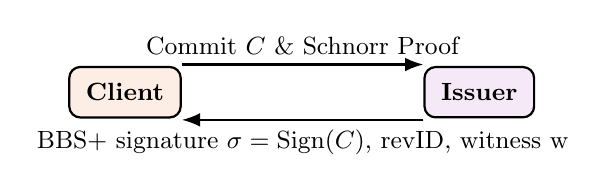
\begin{tikzpicture}[node distance=4.5cm, >=Latex, font=\small]
\node(client)[draw,rounded corners,fill=client!10,thick,inner sep=6pt]{\textbf{Client}};
\node(issuer)[draw,rounded corners,fill=issuer!10,thick,inner sep=6pt,right of=client]{\textbf{Issuer}};

\draw[->,thick] ([yshift=10pt]client.east) -- node[above]{Commit $C$ \& Schnorr Proof} ([yshift=10pt]issuer.west);
\draw[->,thick] ([yshift=-10pt]issuer.west) -- node[below]{BBS+ signature $\sigma = \mathrm{Sign}(C)$, revID, witness w} ([yshift=-10pt]client.east);

\end{tikzpicture}
\end{center}

\textbf{Equations:}\\[-2pt]
  \hspace{30pt}$C = g_1^{m_{\text{birth}}} g_2^{m_{\text{exp}}} g_3^{x_d} h^{r}$,~~
  $\sigma = \text{BBS+Sign}(C)$.
;

\textbf{Client stores:}\\[-2pt]
\begin{itemize}
  \item The issued credential $(C, \sigma, \text{revID}, w)$
  \item The private randomness $r$ and hidden attributes $(m_{\text{birth}}, m_{\text{exp}}, x_d)$
\end{itemize}
\end{frame}


% 5.1 TikZ: Verification Phase — Client-side prep
\begin{frame}{Verification Phase (1/2): Client-side preparation}
\begin{center}
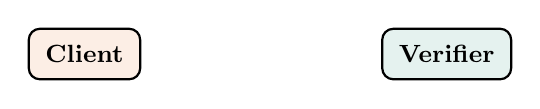
\begin{tikzpicture}[node distance=4.6cm, >=Latex, font=\small]
\node(client)[draw,rounded corners,fill=client!10,thick,inner sep=6pt]{\textbf{Client}};
\node(verifier)[draw,rounded corners,fill=verifier!10,thick,inner sep=6pt,right of=client]{\textbf{Verifier}};
\draw[->,thick,opacity=0] (client.east) -- (verifier.west); % placeholder to keep spacing
\end{tikzpicture}
\end{center}

\textbf{Randomize credential \& initialize proofs}\\[-2pt]
\begin{itemize}
  \item Randomize commitment and signature:
$C' = C \cdot h^{r'}, \quad \sigma' = \text{ReRand}(\sigma, r')$

  \item Prepare BBS+ proof of knowledge (PoK) over hidden attributes
        \((m_{\text{birth}}, m_{\text{exp}}, x_d, r)\).
  \item Set up Bulletproof witnesses:
    \[
      t_{\text{age}} \!=\! \text{age} - \text{threshold},\quad
      t_{\text{exp}} \!=\! \text{expiry\_date} - \text{today}.
    \]
    Target: prove \(t_{\text{age}} \ge 0\) and \(t_{\text{exp}} \ge 0\) via range proofs.
    \item Compute revocation handle $e = $\text{SHA-256}$(x_d)$ and fetch its accumulator witness $w$ to generate a non-membership proof  yet with pedersen: $U = g^e h^r$.

\end{itemize}
\end{frame}

% 5.2 TikZ: Verification Phase — Prover builds & sends proofs
\begin{frame}{Verification Phase (2/2): Build and send proofs}
\begin{center}
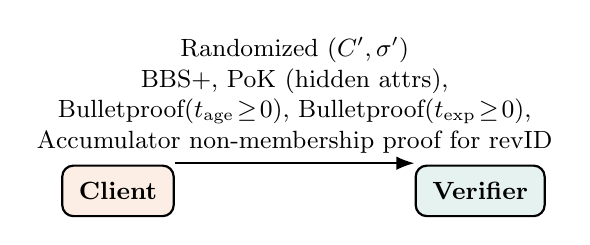
\begin{tikzpicture}[node distance=4.6cm, >=Latex, font=\small]
\node(client)[draw,rounded corners,fill=client!10,thick,inner sep=6pt]{\textbf{Client}};
\node(verifier)[draw,rounded corners,fill=verifier!10,thick,inner sep=6pt,right of=client]{\textbf{Verifier}};

\draw[->,thick] ([yshift=10pt]client.east) -- node[above,align=center]{
  Randomized $(C',\sigma')$\\
  BBS+, PoK (hidden attrs),\\
  Bulletproof$(t_{\text{age}} \!\ge\! 0)$, Bulletproof$(t_{\text{exp}} \!\ge\! 0)$,\\
  Accumulator non-membership proof for \text{revID}
} ([yshift=10pt]verifier.west);
\end{tikzpicture}
\end{center}

\textbf{Proof bundle:}\\[-2pt]
\begin{itemize}
  \item \(\Pi_{\text{BBS+}}\): PoK linking \((C',\sigma')\) to hidden messages. (AND-composed)
  \item \(\Pi_{\text{age}}\): Bulletproof that \(t_{\text{age}} \ge 0\).
  \item \(\Pi_{\text{exp}}\): Bulletproof that \(t_{\text{exp}} \ge 0\).
  \item \(\Pi_{\text{acc}}\): Non-membership of \(\text{revID}\) in accumulator.
\end{itemize}
\end{frame}


% 5. System Entities Overview
\begin{frame}{System Overview (Entities \& Roles)}

\begin{center}
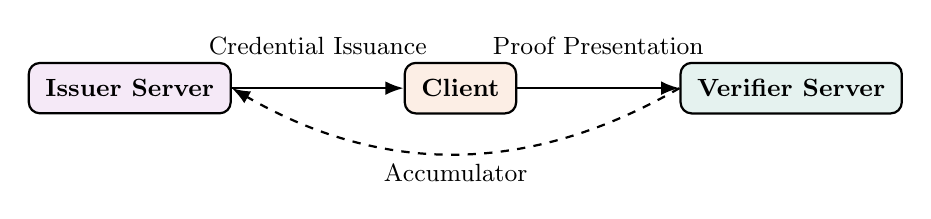
\begin{tikzpicture}[node distance=4.2cm, >=Latex, font=\small]
\node(issuer)[draw,rounded corners,fill=issuer!10,thick,inner sep=6pt]{\textbf{Issuer Server}};
\node(client)[draw,rounded corners,fill=client!10,thick,inner sep=6pt,right of=issuer]{\textbf{Client}};
\node(verifier)[draw,rounded corners,fill=verifier!10,thick,inner sep=6pt,right of=client]{\textbf{Verifier Server}};

% Arrows
\draw[->,thick] (issuer.east) -- node[above,yshift=0.3cm]{Credential Issuance} (client.west);
\draw[->,thick] (client.east) -- node[above,yshift=0.3cm]{Proof Presentation} (verifier.west);

\draw[->,thick,dashed] (verifier.west) to[bend left=30] node[below]{Accumulator} (issuer.east);
\end{tikzpicture}
\end{center}

\medskip
\textbf{Roles:}
\begin{itemize}
  \item \textbf{Issuer:} Issues credentials, manages RSA accumulator (revocation list), publishes public parameters.
  \item \textbf{Client:} Holds credentials, generates ZK proofs (BBS+, Bulletproofs, revocation).
  \item \textbf{Verifier:} Validates proofs, checks non-revocation.
\end{itemize}

\end{frame}


% 6. System Design / Implementation
\begin{frame}{System Design \& Implementation}
\begin{columns}[T,onlytextwidth]
\column{0.55\textwidth}
\textbf{Architecture}
\begin{itemize}
  \item All components in \textbf{Go}; lightweight REST APIs; thin JS UI.
  \item Client runs local Go backend; cryptography stays off the browser.
  \item Verifier caches issuer params; enforces freshness \& replay protection.
\end{itemize}
\column{0.45\textwidth}
\textbf{Packages}
\begin{itemize}
  \item \texttt{pkg/crypto}: Pedersen, BBS+ on BLS12-381.
  \item \texttt{pkg/protocol}: Bulletproofs, serialization, verification.
  \item \texttt{pkg/revocation}: RSA accumulator, witnesses.
\end{itemize}
\end{columns}
\end{frame}

% 7. Security & Performance
\begin{frame}{Security \& Performance (Highlights)}
\begin{itemize}
  \item \textbf{Zero-knowledge}: proofs reveal no personal data.
  \item \textbf{Unlinkability}: re-randomization; no static identifiers.
  \item \textbf{Unforgeability}: BBS+ on BLS12-381.
  \item \textbf{Revocation privacy}: only revoked IDs in accumulator.
\end{itemize}
\end{frame}

% % 8. Comparison Table
% \begin{frame}{Comparison}
% \begin{center}
% \begin{tabular}{lccc}
% \toprule
% Method & Privacy & Linkability & Setup \\
% \midrule
% ID Upload & Low & High & None \\
% Credit Check & Low & High & None \\
% zkSNARKs & High & Low & Trusted \\
% \textbf{Our System} & \textbf{High} & \textbf{None} & \textbf{None} \\
% \bottomrule
% \end{tabular}
% \end{center}
% \end{frame}

% 9. Future Work
\begin{frame}{Future Work}
\begin{itemize}
  \item Bind credentials to device secrets/biometrics for anti-sharing.
  \item Native mobile SDKs (Android, iOS).
  \item Threshold issuers and decentralized identifiers.
  \item Cross-authority scaling with common identifiers.
\end{itemize}
\end{frame}

% 10. Conclusion
\begin{frame}{Conclusion}
\begin{itemize}
  \item Practical, privacy-preserving age checks without identity disclosure.
  \item Compact ZK composition: Pedersen + BBS+ + Bulletproofs + RSA accumulator.
  \item Efficient on BLS12-381 with a clean Go-based architecture.
\end{itemize}
\end{frame}

\end{document}
